\subsection{Queries}\label{sec:queries}
We have created several queries in order to verify the schedule and output relevant data. We want to verity that we do not fall below the battery threshold, and the payloads that are scheduled are executed. Additionally, we want to monitor other variables in order to present the user with all the relevant data we are able to extract, such as the accumulated profit.

% impotant
\begin{equation} \label{eq:smc2}
	Pr\; [<=ScheduleLength] \; (<>\; a\ <\ a\ *(Threshold/100))
\end{equation}
Query \ref{eq:smc2} will result in a probability that reflects the risk of the battery going below the threshold. This threshold is specified in the configuration file from \cref{subsec:init} \nameref{subsec:init}. This is as previously mentioned a state which may not occur, as it would cause the nanosatellite to enter a safe mode where it is not possible to communicate with it.

It is expected that battery usage in the \gls{smc} model differs from that in the \gls{cora} model as they use two different battery models, Ideal and \gls{kibam}. The usage may also vary because of the possible difference in time usage that the individual payloads takes to complete. The time it takes to complete one payload in \gls{cora} are constant but in \gls{smc}it may vary, as we want to model the uncertainty.

We expect that we will use less energy in the \gls{smc} model because \gls{kibam} under estimates the energy consumption whereas the model used in \gls{cora} will overestimate. The \gls{smc} model is also guaranteed to use the same amount, or less, time to complete a payload than \gls{cora}. This is due to \gls{cora} model using the worst case time when executing the payloads.

% impotant
\begin{equation} \label{eq:smc3}
	Pr\; [<=ScheduleLength] \; (<> \ skips \ !=\ 0)
\end{equation}
Query \ref{eq:smc3} are used for finding the chance of all scheduled payloads are run. The reason for it not doing so may vary but it will often be as a result of a untimely restart of the system or a different battery level than expected due to the more precise battery model implemented in the \gls{smc} model.

% extra
\begin{equation} \label{eq:smc4}
	simulate\ 100 \; [<=ScheduleLength] \; \{active, \; Processor.Running\}
\end{equation}
Query \ref{eq:smc4} is used to output the order of payloads that was executed. This should correspond to the order that the trace from \gls{cora} dictates, but there could be differences if it was necessary to skip a payload. This query becomes especially relevant in cases where query \ref{eq:smc3} returns a chance of payloads being skipped. The output of query \ref{eq:smc4} will allow us to see exactly which payloads was skipped at what time.

\begin{figure}[H]%
	\centering
	\subfloat
	{{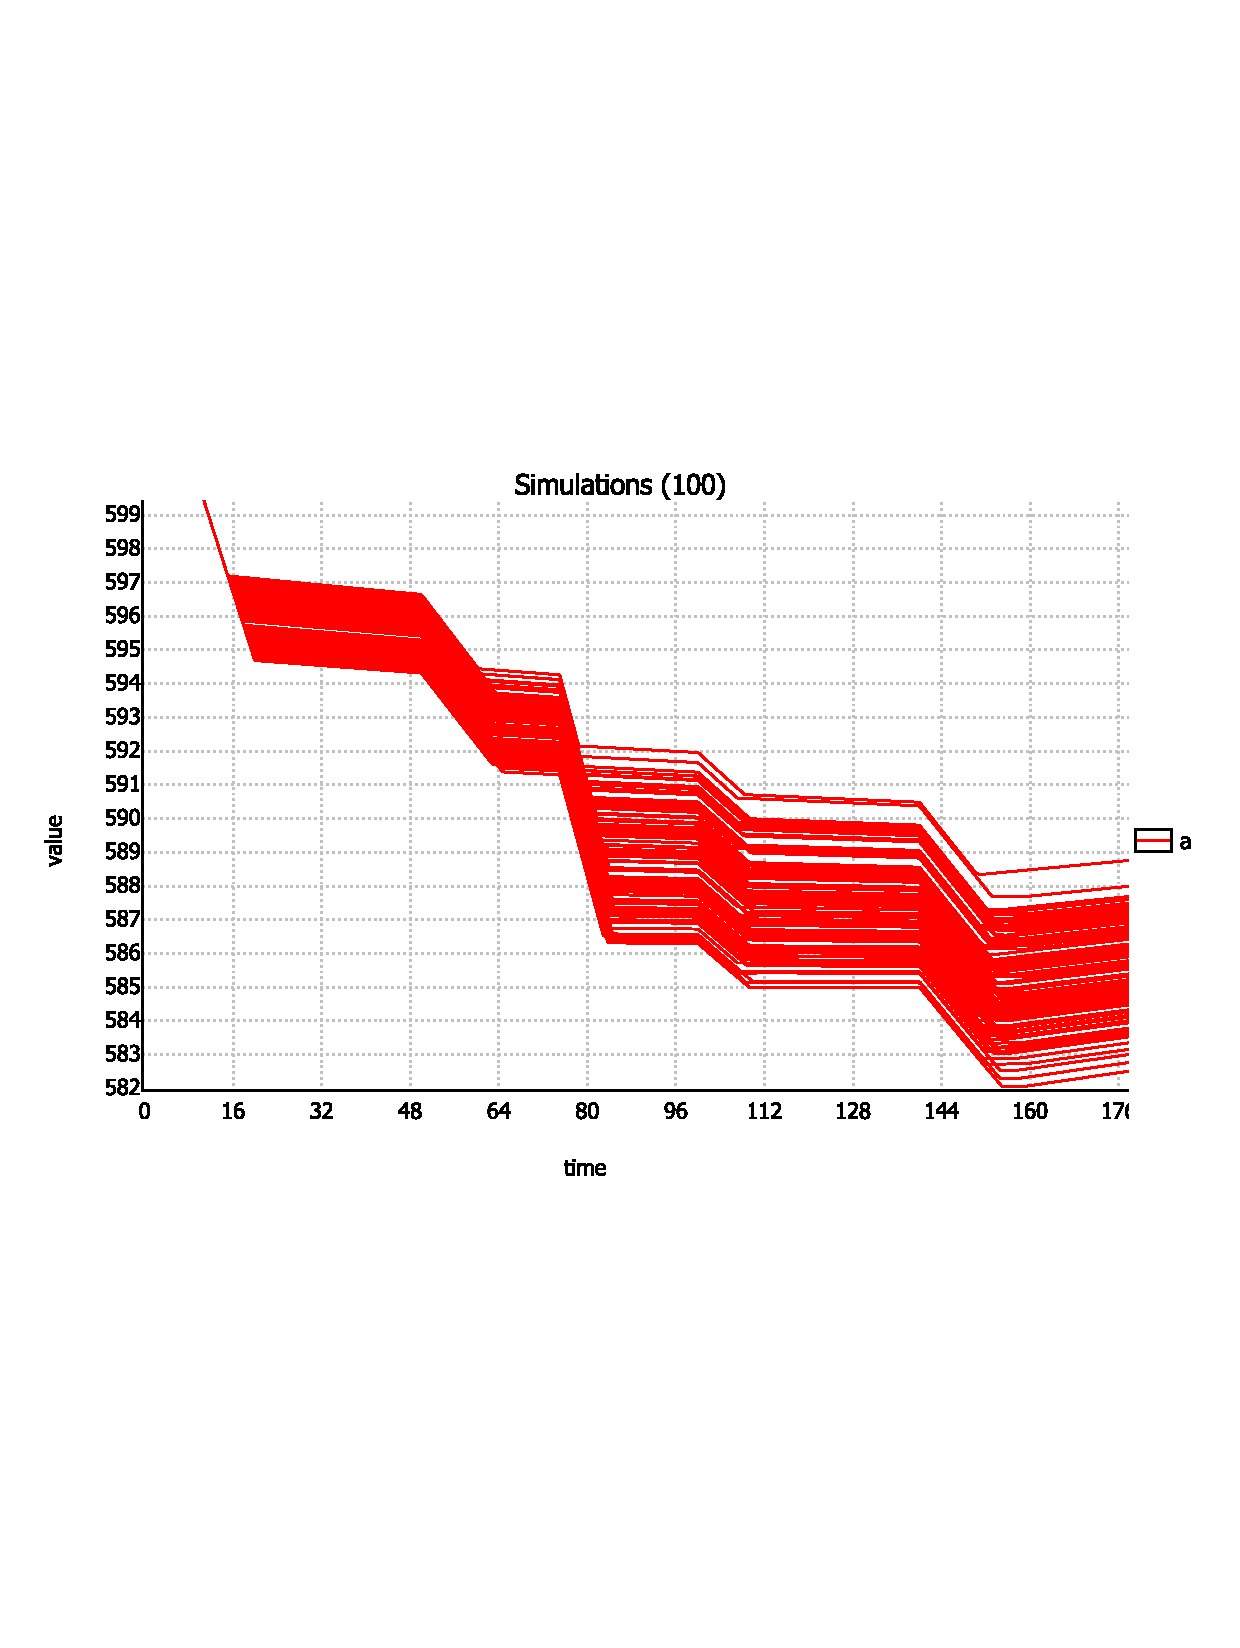
\includegraphics[width=7cm, trim={0 8cm 0 6cm},clip] {graphics/simulation_graphs/SimulationsA100.pdf} }}%
	\qquad
	\subfloat
	{{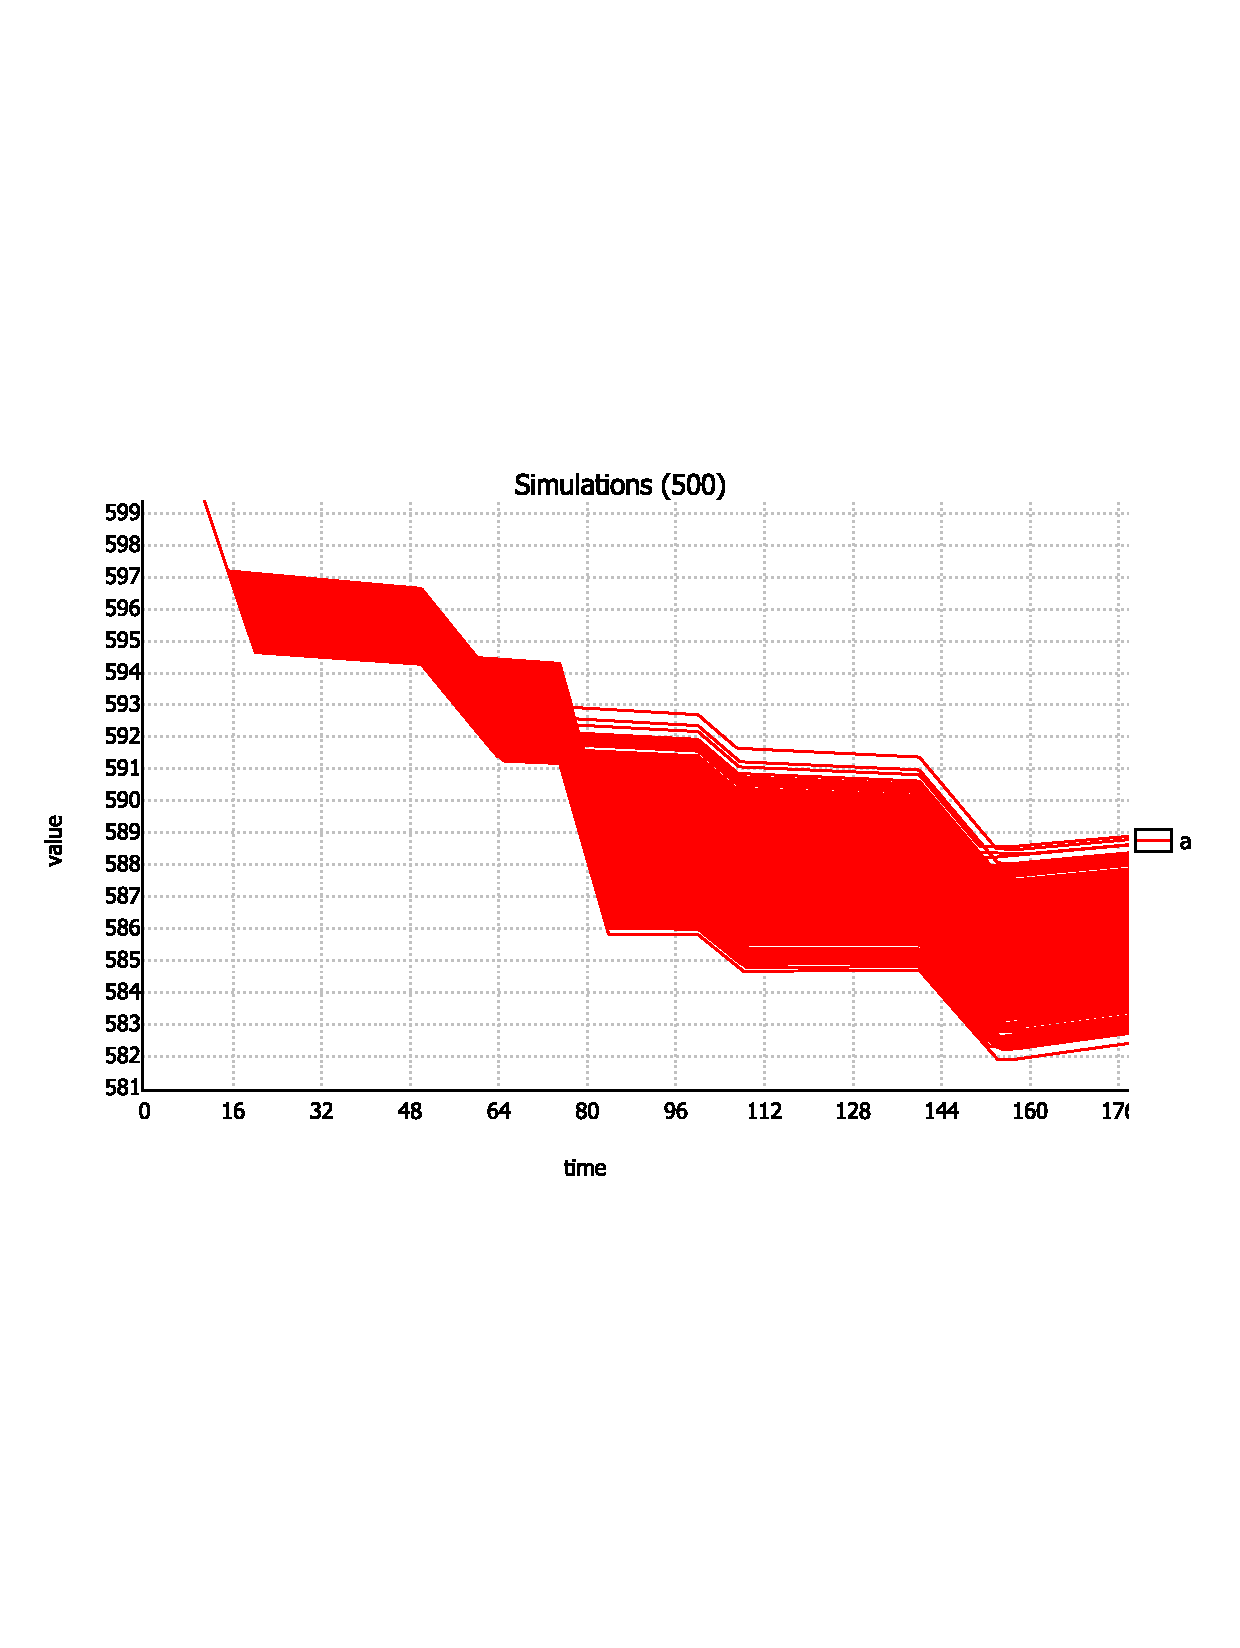
\includegraphics[width=7cm, trim={0 8cm 0 6cm},clip] {graphics/simulation_graphs/SimulationsA500.pdf} }}%
	\caption{100 simulations(left) versus 500 simulations(right) over available energy \textit{a} in smc}%
	\label{fig:sim_amount}%
\end{figure}
In query \ref{eq:smc4} it is specified that we want to run the simulation 100 times, the reason for this is that we consider 100 simulations is adequate to give a reasonable representation of the values range. In \cref{fig:sim_amount} we see two graphs, one where the simulation have been run 100 times and one where it have been run 500 times. It can there be seen that the lowest observed value of \textit{a} is similar in both graphs, $182$ in the one with 100 simulations and $181.9$ in the one with 500 simulations. And the highest value observed by the end of the simulations were $188.8$ versus $189$. In both cases the 500 simulations displays a wider range for the value, however the query running 100 simulations took 9 seconds, whereas the one with 500 took $55$ seconds.\\
With the small differences to the final output and the large amount of time saved we conclude that running 100 simulations will give an acceptable range in short time. Therefore we will use 100 simulations for all queries of the type simulation.

\begin{equation} \label{eq:smc5}
	simulate\ 100 \; [<=\ ScheduleLength]\; \{ a,\ b\}
\end{equation}
Query \ref{eq:smc5} provides two time series that reflects the two wells, a and b, from the battery. This is useful for the user as they might want to discard the schedule if it uses more energy than what they are comfortable with. Even if we do not go below the threshold, it may be to expensive to execute the schedule. % forklar hvorfor at vi kører 10 simulations?

% extra
\begin{equation} \label{eq:smc6}
	E \; [<=\ ScheduleLength;\ 100]\; ( max:\ earnings)
\end{equation}
Query \ref{eq:smc6} shows the accumulated profit for the schedule, and was introduced in \cref{subsec:csv} \nameref{subsec:csv}. We will not judge a schedule based on this value, we will let the user decide if it is acceptable. The profit is a abstract variable and we will not be able tell whether or not it is satisfactory.


The three last queries, \ref{eq:smc4}, \ref{eq:smc5}, and \ref{eq:smc6}, are tested with simulations. The simulations are great for giving the user insight in the behaviour of the nanosatellite when executing the schedule. \\
It does however not set any guarantees for the correctness or robustness of the schedule as it only displays the result of the path taken during each of the simulations.


\ofx{NOTE:}%for at få den endelige battery cap hvad kan vi gøre?
%	- similate x [<= schedule_length]{a} tag end value af "a" for hvert run og udregn average worst og lowest
%	- Pr [<= schedule_length] {a in range x to x+y}
%	- Pr [<= schedule] {average a +- 10%}

\subsection{Parameter Tuning}

